\chapter{Marco de Referencia}

 Desde finales del siglo pasado, los avances tecnológicos en la miniaturización de la electrónica y los componentes mecánicos han allanado el camino para la creación y desarrollo de objetos voladores de pequeñas dimensiones, tales como aviones y helicópteros, los cuales están adquiriendo cada vez más habilidades para realizar vuelos de forma autónoma. Estos dispositivos son popularmente conocidos como drones, un término derivado del inglés \say{abejorros}, y se consideran máquinas voladoras autónomas o semi-autónomas capaces de llevar a cabo misiones de vuelo. En el ámbito internacional, se les conoce como UAVs del ingles \say{Unmanned Aerial Vehicles}, y representan una tecnología compleja cuyo control presenta desafíos, dado que sus características aerodinámicas son similares a las de las aeronaves convencionales \cite{eisenbeiss2004mini}.

El estudio de estos dispositivos despierta un gran interés debido a su versatilidad y capacidad de maniobra, lo que les permite llevar a cabo una amplia gama de tareas en diversas aplicaciones, tales como el uso civil, militar y aeroespacial \cite{nawaz2019applications, shakhatreh2019unmanned, xiaoning2020analysis}. En la figura \ref{fig1_aplicacion_UAV}, se presenta una clasificación detallada de las aplicaciones más importantes de los UAVs.

\begin{figure}[H]
    \centering
    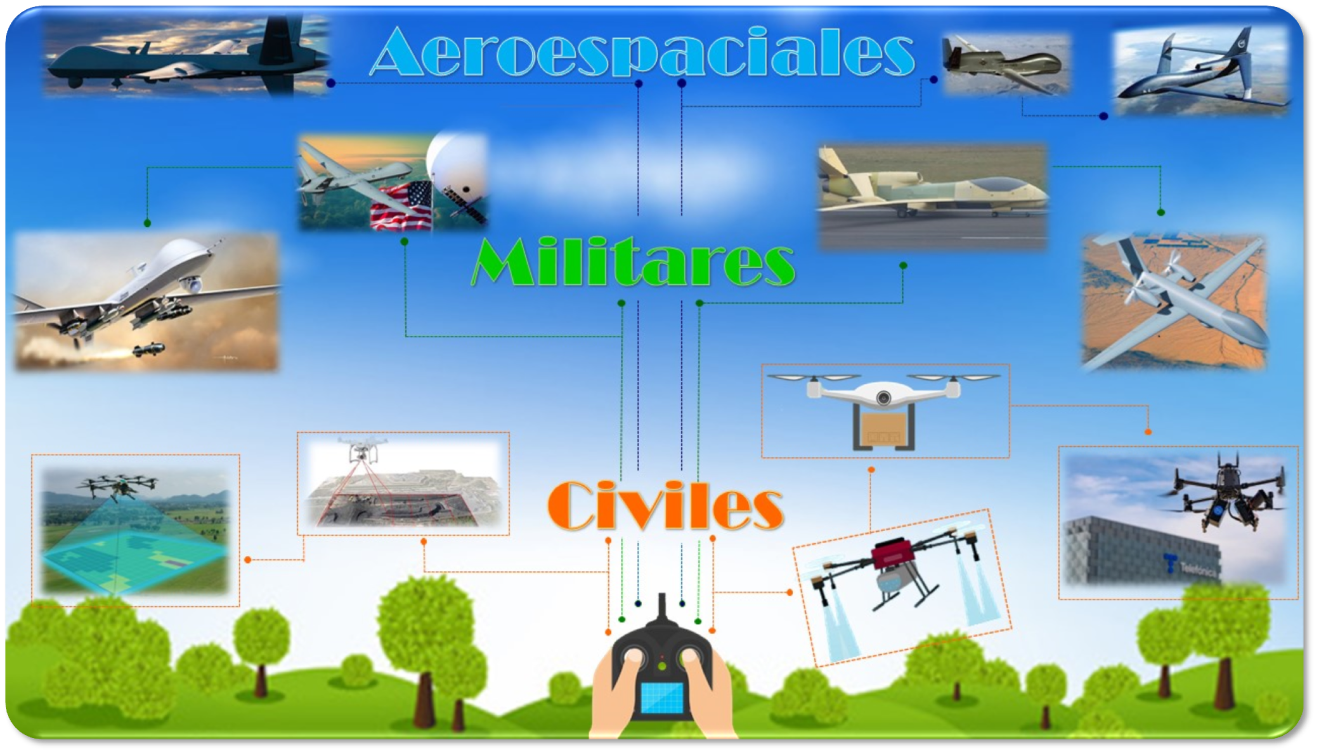
\includegraphics[width=16cm, height=7.5cm]{imagenes/Aplicaciones_UAV.png}
    \caption{Áreas de aplicación UAVS.}
    \label{fig1_aplicacion_UAV}
\end{figure}

\section{Antecedentes.}

Los drones han atraído la atención de la comunidad investigadora que trabaja tanto en el campo militar como en el civil, con una gran cantidad de usos que han sido propuestos por los grupos de investigación, debido a sus características como capacidad y configuraciones, donde el helicóptero de cuatro rotores tiene el mayor número de citas en la literatura de control y ha sido ampliamente investigado para pruebas tanto en interiores como en exteriores . 

\section{Objetivo General}
\textbf{}
\section{Objetivos Especificos}
\begin{enumerate}

\section{Objetivo General}

Desarrollar un sistema web de gestión de cursos e inscripciones en línea para la optimización de los procesos académicos y administrativos de instituciones de capacitación, mediante el framework Laravel, una base de datos MariaDB y una arquitectura Modelo-Vista-Controlador (MVC) complementada con una capa de servicios y mecanismos de control de acceso basados en roles y permisos.

\section{Objetivos Específicos}

\begin{enumerate}

    \item \textbf{Analizar} los requerimientos funcionales y no funcionales del sistema para la definición de las reglas de negocio relacionadas con usuarios, cursos, inscripciones, pagos y seguimiento académico, mediante la identificación y clasificación de las necesidades de los distintos tipos de usuarios.

    \item \textbf{Diseñar} la arquitectura MVC del sistema, el modelo entidad-relación de la base de datos y las interfaces de usuario para la organización de la información y la estructura de los procesos, mediante diagramas, prototipos y la definición de relaciones entre entidades.

    \item \textbf{Implementar} los módulos funcionales del sistema para la automatización y validación de los procesos académicos y administrativos, mediante Laravel, MariaDB, una capa de servicios, middleware de autorización y pruebas automatizadas.

    \item \textbf{Verificar} el funcionamiento de los módulos del sistema y el cumplimiento de las reglas de negocio para la detección de errores y la comprobación de su correcto comportamiento, mediante pruebas unitarias, de integración y funcionales.

    \item \textbf{Documentar} la estructura técnica y los procedimientos de operación del sistema para facilitar su comprensión, mantenimiento y utilización, mediante la elaboración de manuales, diagramas y registros de las funcionalidades implementadas.

    \item \textbf{Desplegar} el sistema web en un entorno de ejecución controlado para la comprobación de su disponibilidad y funcionamiento integral, mediante la configuración del servidor, la base de datos y los servicios necesarios para su operación.

\end{enumerate}


\section{Alcance}

El proyecto contempla el desarrollo de un sistema web para la gestión de cursos e inscripciones en línea, dirigido a instituciones de capacitación que requieran centralizar sus procesos académicos y administrativos. La plataforma permitirá la administración de usuarios, cursos, grupos, inscripciones, materiales educativos, evaluaciones, pagos y constancias digitales.

El sistema contará con cinco roles principales: administrador, coordinador, recepción, instructor y participante, cada uno con permisos específicos de acuerdo con sus responsabilidades. Asimismo, incorporará mecanismos de autenticación y autorización, validación de requisitos, control de cupos y seguimiento del desempeño académico de los participantes.

La aplicación estará orientada a cursos virtuales, tanto autogestionados como acompañados por instructores, y se desarrollará mediante el framework Laravel, bajo una arquitectura Modelo-Vista-Controlador (MVC) complementada con una capa de servicios y una base de datos MariaDB. Su funcionamiento se verificará mediante pruebas automatizadas para comprobar el cumplimiento de las principales reglas de negocio.

\section{Limitación}

El sistema estará orientado exclusivamente a la administración de cursos en modalidad virtual, por lo que no contemplará la gestión de aulas físicas, instalaciones educativas ni actividades académicas presenciales.

Su funcionamiento dependerá de una conexión a internet y de la disponibilidad de la infraestructura tecnológica donde se encuentre alojado. Asimismo, el rendimiento y la capacidad de atención simultánea estarán sujetos a los recursos del servidor y a la configuración del entorno de despliegue.

El registro de cuentas de usuario estará restringido al personal autorizado, por lo que los solicitantes no podrán crear cuentas directamente sin un proceso previo de revisión y aprobación. Además, la plataforma no desarrollará herramientas propias de videoconferencia, sino que podrá utilizar enlaces a servicios externos para las sesiones virtuales.

Finalmente, las pruebas del sistema se realizarán en un entorno controlado, por lo que sus resultados permitirán verificar el comportamiento de las funcionalidades implementadas, sin garantizar el mismo rendimiento bajo todas las condiciones posibles de operación.

\section{Problemática}


\section{Justificación}

